\chapter{Background}
\label{chap:background}

This work centers around investigating and improving the quality of corrupted communications in low power networks.
Therefore this chapter will provide the necessary background information on the form of communication used in \acl{WSN}s and the radio and microcontroller hardware we employed in our study.
Furthermore, we describe the theory of operation of \acl{FEC} and shortly describe what approaches to \acl{ECC}s exist and how they work.

\section{\acl{WSN}s}

A \acf{WSN} comprises of two or more nodes, called \emph{motes}, which can communicate using low power radio communication.
This provides a means to easily deploy sensing, actuating and communication infrastructures in a given space.
The nodes are mostly powered by small and simple microcontrollers connected to a radio and other peripherals such as sensors and actuators as shown in Figure~\ref{fig:mote_schematic}.

Networked motes communicate with their neighboring motes and can address the whole network via multi-hop transmissions, therefore deprecating the use of expensive wired buses.
However, due to the nature of wireless communication, the software must be built to tolerate unreliable communication links, which can change network topology and result in high latency in data exchanges or a complete loss of communication.

Integrated batteries are used to power the motes for a certain amount of time when deployed in areas where access to a power grid is too costly or impossible.
Especially for these battery powered applications, conserving energy is a high priority and places tight restrictions on the type of CPU and radio transmission power and duty cycle, effectively limiting communication range and bandwidth.

A typical application for a \ac{WSN} would be the collection of meteorological information over large inaccessible areas, such as forests, or the monitoring of large industrial complexes to reduce the cost of wiring~\cite{Boano2009}.
The high effort required to exchange empty batteries in these scenarios demands energy-aware programming, which keeps the overall energy consumption to a minimum.

\begin{figure}[t]
	\tikzset{
		boxt/.style={
	           rectangle,
	           fill=white,
	           draw=black, thick,
	           text width=2cm,
	           minimum height=1cm,
	           text centered},
	}
	\centering
	\begin{tikzpicture}[>=stealth',
	<->,
	shorten <=1pt,
	shorten >=1pt]
		% \draw (0,0) rectangle (7,5);
		\node[boxt, fill=slightgray] (controller) at (4, 4.3) {$\mu$Controller};
		\node[boxt] (sensors) at (5.7, 2.8) {Sensors};
		\node[boxt] (actuators) at (5.7, 1.7) {Actuators};
		\node[boxt, fill=slightgray] (radio) at (2.3, 1.7) {Radio};
		\node[boxt] (storage) at (2.3, 2.8) {Storage};
		\node (antenna) at (0.4, 3.5) {};
		\node[font=\small] (uart) at (6.35, 4.65) {UART};

		\draw (1,1) rectangle (7,5);
		\draw[thick] (1,0) rectangle (7,0.9) node[midway] {Power Source};

		\draw[thick] (controller.east) -| (sensors.north);
		\draw[thick] (controller.west) -| (storage.north);
		\draw[thick] ($(controller.south west)!0.45!(controller.south east)$) |- (radio.east);
		\draw[thick] ($(controller.south west)!0.55!(controller.south east)$) |- (actuators.west);
		\draw[thick, ->] ($(controller.south east)!0.8375!(controller.north east)$) -- (uart.west);

		\draw[very thick, -, shorten <=0pt, shorten >=-3pt] (radio) -| (antenna);
		\fill[color=black] (antenna) circle (0.075);
		\draw[dashed] (antenna) circle (0.15);
		\draw[dashed] (antenna) circle (0.25);
		\draw[dashed] (antenna) circle (0.35);
		\draw[dashed] (antenna) circle (0.45);

	\end{tikzpicture}
	\caption{A schematic representation of a mobile \acs{WSN} mote with a power source.}
	\label{fig:mote_schematic}
\end{figure}


\section{Communications}

Since this works focuses heavily on communications between motes, we use specific terms to help describe its properties.

A \emph{packet} is the basic unit of communication between two motes, containing metadata, such as sender and addressee, and payload.
A \emph{message} is the interpretation of the payload of one or several packets.
If a message is very long, it might be fragmented into several packets, however, in all our experiments, one message uses only one packet.
We define a \emph{link} as the transmission of messages from one mote addressed to another over a period of time, even when none of these messages where received by the addressee, due to channel effects or connection problems.


\subsection{IEEE 802.15.4 Standard}

In this work we use the CC2420 wireless transceiver~\cite{cc2420}, a very common communication radio in \acp{WSN}.
The CC2420 implements the \ac{IEEE} 802.15.4 standard and uses \ac{OQPSK} modulation in the \SI{2.4}{\giga\hertz} ISM band with a nominal data rate of \SI{250}{\kilo bit\per\second}.

The \ac{PPDU} is the lowest accessible layer as shown in Figure~\ref{fig:packet_format} with a maximum size of 133 bytes.
This leaves 127 bytes for the \ac{MPDU} and between 102 and 122 bytes for the frame payload.
To increase robustness of transmission, each byte is split into two 4-bit symbols, which are then mapped to a 32-bit chip sequence and modulated using \ac{OQPSK}.

These 32-bit chip sequences are part of \ac{IEEE} 802.15.4 and were chosen to produce high Hamming distances against each other, so that bit errors can already be corrected within the received chip sequence to some degree. 
The higher the Hamming distance between two sequences, the less likely they are to be mistaken for one another.
Therefore a corrupted 4-bit symbol is only received, when a corrupted chip sequence is mistaken for another sequence, which requires several bits of the 32-bit sequence to be flipped.
The minimum Hamming distance between two sequences is 12 bit, the maximum is 20 bit~\cite{Schmidt2013}.

At the beginning of every transmission, a Preamble Sequence is modulated, which triggers a listening mote to synchronize and receive this new packet.
Typical reasons for not receiving packets are either the reception of a signal with too little power to be noticeable above the channel noise, or the reception of a corrupted preamble, so that the listening mote does not start receiving a packet, even though the power levels would permit it.

When a packet is received, its \ac{FCS} is automatically evaluated to check for bit errors introduced by channel noise.
However, a failed \ac{FCS} test can also be the results of a corrupted Frame Length field.
This prompts the radio to read in too few or too many bytes, thereby comparing the \ac{FCS} results to the wrong bytes at, what the receiver wrongly considers the ``end'' of the packet.

Even though the \ac{FCS} is evaluated for all messages automatically, the CC2420 allows retrieval of corrupted messages, including all hardware link qualifiers such as \ac{LQI} and \ac{RSSI}.
We make use of this ability to analyze the content of these corrupted messages in our work.

\begin{figure}[t]
	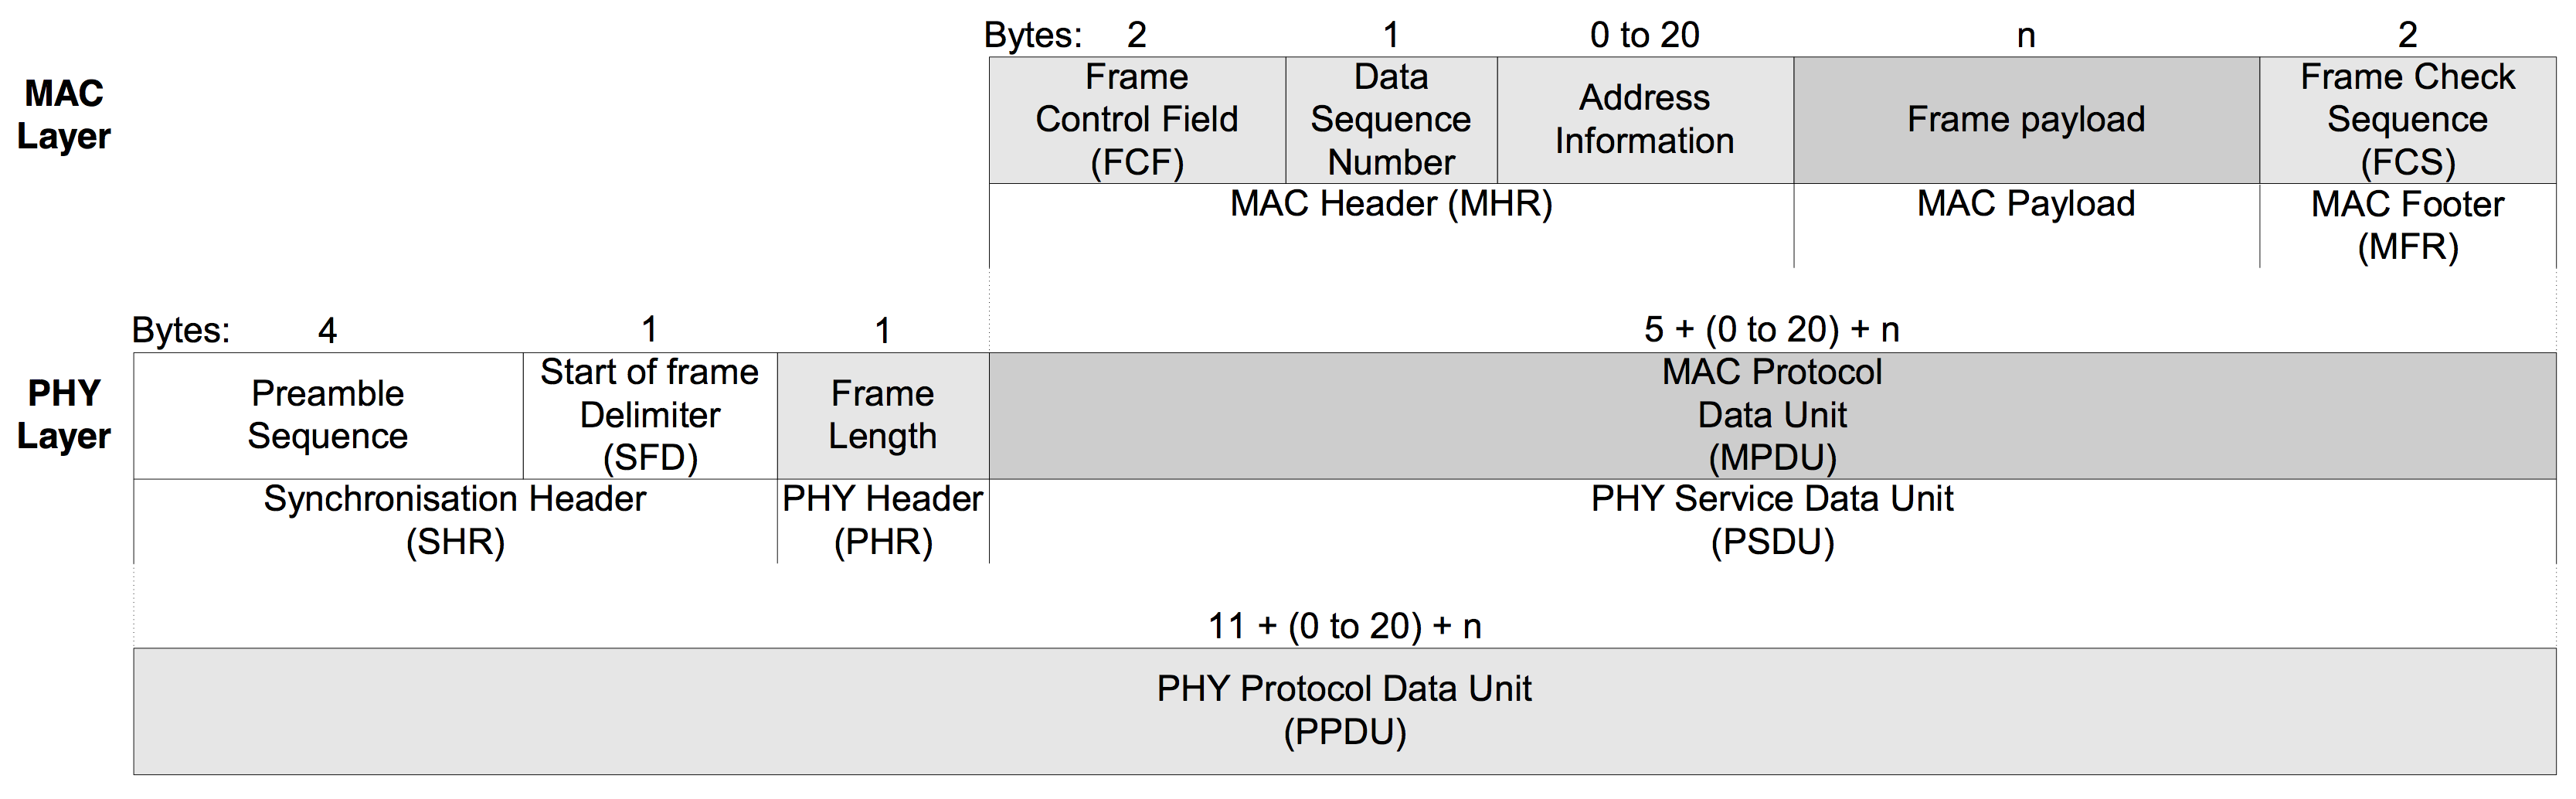
\includegraphics[width=1\columnwidth]{figures/frame_format}
	\caption{The packet format implemented defined by \acs{IEEE} 802.15.4 taken from \cite{cc2420}.}
	\label{fig:packet_format}
\end{figure}

\subsection{\acs{UART} Communication}

The microcontroller can also communicate over a wired bus using its \ac{UART} module.
\ac{UART} does not provide a seperate clock line (hence \emph{asynchronous}), which requires the receiver to synchronize itself at the beginning of each symbol transfer and sample the signal at multiples of the baudtime $t_{symbol} = f_{Clock} / f_{BaudRate}$, which derives from the \emph{baudrate} of the transmitter.
Here the receiver synchronizes on the falling edge of the start bit, which is always low, and has to sample the successive bits at the just right time, as shown in Figure~\ref{fig:uart_timing}.
If the transmitter's and/or receiver's clock is running too slow or too fast, then $t_{Symbol}$ is too small or too large, resulting in a corrupted sampling of the bits in the symbol as marked in red.

The relative error tolerance for the 8N1 configuration shown in the Figure (8 databits, 1 startbit and 1 stopbit) is $\pm5\%$, since the sample point of the stop bit may only shift by at most $\pm t_{Symbol}/2$.
With 10 bits to read, one $t_{Symbol}$ equals one tenth of the symbol transmission time, hence a relative tolerance of $\pm5\%$.
For example, the tolerance for 7-bit transfers (9 baudtimes) increases to $\pm5.56\%$.

However, since both transmitter and receiver may experience clock drift, the error must not exceed $5\%$ in total, which in the worst case of opposing clock drift directions (one too fast, one too slow) imposes a tight allowed deviation of $+2.5\%$ and $-2.5\%$ on the modules respectively.
In practice, \ac{UART} can therefore be difficult to use with uncorrected or unknown clock drifts.

\begin{figure}[t]
	% \centering
	\begin{tikzpicture}[thick, >=stealth']
		\draw[white] (-4.5,-0.75) -- (-3,-0.75);

		\def \di {0.46}
		\def \dii {0.535}

		\fill[slightgray] (1,2) rectangle (1.5,3) node[midway, black] {S};
		\fill[slightgray] (5.5,2) rectangle (6,3) node[midway, black] {P};

		\foreach \s in {0,...,7}
		{
			\draw (1.5+\s*0.5,2) rectangle (2+\s*0.5,3) node[midway] {\s};
		}

		\draw[-] (-1,3) -- (1,3) -- (1,2) -- (1.5,2);
		\draw[-] (5.5,3) -- (8,3);

		\path (-1,2) -- (1,3) node[midway, font=\tiny] {\textbf{IDLE}};
		\path (6,2) -- (8,3) node[midway, font=\tiny] {\textbf{IDLE}};

		\draw[->] (2.5,3.75) -- (7,3.75) node[midway, above, font=\small] {Time};

		\draw[->, shorten <=1pt, shorten >=1pt] (1,3.5) node[above, font=\small] {Sync} -- (1,3);

		\foreach \s in {0,...,9}
		{
			\filldraw (1.25+\s*0.5, 1.2) circle (0.06);
		}

		\draw[|<->|, shorten >=-0.4pt, shorten <=-0.4pt] (1,1.6) node[left=0pt, font=\small] {$t_{Symbol}$} -- (1.5,1.6);
		\draw[->, shorten >=3pt] (6.1, 1.65) node[right=0pt, font=\small] {Ideal Timing} -| (5.75, 1.2);


		\node[font=\small, right] at (-1,0.5) {Too Fast};
		\node[font=\small, right] at (-1,-0.2) {Too Slow};

		\fill[slightred, rounded corners] (1.25+\di*4.5+\di-0.5, 0.3) rectangle (1.25+\di*9.5+\di-0.5, 0.7);
		\foreach \s in {0,...,9}
		{
			\draw (1.25+\s*\di+\di-0.5, 0.5) circle (0.06);
		}

		\fill[slightred, rounded corners] (1.25+\dii*5.5+\dii-0.5, -0.4) rectangle (1.25+\dii*9.5+\dii-0.5, 0);
		\foreach \s in {0,...,9}
		{
			\draw (1.25+\s*\dii+\dii-0.5, -0.2) circle (0.06);
		}

		\foreach \s in {0,...,10}
		{
			\draw[line width=0.2pt] (1+\s*0.5,1.9) -- (1+\s*0.5,-0.6);
		}
	\end{tikzpicture}
	\caption{\acs{UART} timing diagram of the sampling points of an 8-bit symbol.}
	\label{fig:uart_timing}
\end{figure}

\section{Error Control Schemes}

There exist two approaches to improve the quality of an imperfect communication channel: using \ac{FEC} to add redundancy before transmission, so that bit errors can be \emph{detected} and \emph{corrected} by the receiver, and using \ac{ARQ} to only \emph{detect} bit errors, but request a retransmission, instead of correcting them.
While \ac{ARQ} is simple and requires very little computational and transmission overhead, it does perform poorly in conditions with a high channel error rate.
\ac{FEC} allows constant throughput at the expense of coding and decoding time and transmission overhead, depending on the specific \ac{ECC} used.
To overcome their individual disadvantages, these two approaches can be merged into \emph{hybrid} \ac{ARQ} schemes, however, in our work we will be focusing on using \ac{FEC} schemes alone.

The simplest \acp{ECC} belong to the class of linear cyclic coding schemes, where a bit stream is divided into non-overlapping blocks, which are then encoded separately.
The most widely used linear cyclic block codes are binary \ac{BCH} and non-binary \ac{RS} codes, both of which can be used to correct bit and burst errors.
There are several other approaches to \acp{ECC}, however, they go above the focus of this work.



